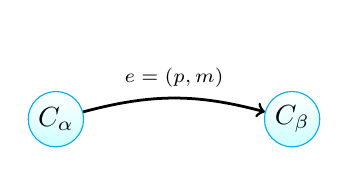
\begin{tikzpicture}[scale=1.5]
\tikzset{nodo/.style={circle,minimum size=20pt,inner sep=0pt,draw, top color=white ,bottom color=cyan!20, cyan,text=black}}
\tikzset{nodo1/.style={circle,minimum size=20pt,inner sep=0pt, color=black}}

  \draw (0,0) node[nodo](p) {$C_{\alpha}$};
  \draw (2,0) node[nodo] (q){$C_{\beta}$}; 
  \draw(1,0.35) node[nodo1](e){\scriptsize{$e=(p,m)$}};
  
  \draw [->, line width=1pt] (p) to [bend left=15] (q);
    
 \end{tikzpicture}
 